% Data source: benchmark/analysis/outputs/windows-native-v1/delivery-review.json
% Scientific source: 0c9325e98f2bc7dcd75d344c01c2e50a62801c90
% Protocol identity: 1d233dd09956c4575fc5775082310e5edca65407db5fcef40bc2ce329e6f5898
% The received Windows evidence was independently reviewed on Mac; see docs/WINDOWS-RETURN-AUDIT.md.
\section{原生Windows扩展：独立开发版本与新冻结实验}
\label{sec:windows-native}

开发分支\texttt{windows-native-dev}新增Python版本0.2.0.dev1及R版本0.2.0.9001。
明确torch目标与独立NumPy参考可在不导入JAX的条件下运行，基础安装不再强制拉取JAX。
本轮实际环境为Windows 11、AMD Ryzen 7 9800X3D、NVIDIA RTX 5080（sm\_120）、
驱动616.56、Python 3.12.14、torch 2.13.0+cu130及float64。
R 4.6.1通过reticulate整批调用并保持iteration$\times$chain$\times$variable次序。
Stan仍为CPU提供方式，未自动翻译；本轮未编译核验原生Stan。
Pyro 1.9.2的CPU NUTS仅作为单独正态目标统计基线，未接入GPU NUTS。

实现保持相同MALA/RWM核约定、硬接受前向、独立参考与实际随机数组。
quasi-DEER使用非重叠窗口和截断Rademacher对角JVP；Picard使用滑动窗口，
多链按最小已确认前缀共同推进，末窗口只处理实际转移。
控制采用torch eager与Python循环，记录主机标量等待，不宣称融合设备内控制。
CPU 65项和CUDA 63项测试通过，另有72项原始路径比较与8个R批量核验。
这些有限测试不构成一般正确性证明。

试探网格96项完成后，在观察正式结果前冻结\texttt{windows-native-v1}。
协议包含8个目标、128/512两个预算、每组4份独立随机数组、CPU/CUDA资源和4个MH工作流，共512项，
每项4链、窗口16。新身份同时锁定源码、依赖、设备、数据、数组、坐标、函数与失败规则。
所有512项通过数值输出检查，接受事件对独立NumPy参考零失配，最大路径差为$@ORACLE_ERROR@$。
256对CPU/CUDA实际数组比较亦无事件失配，最大无约束及约束差分别为
$@DEVICE_PATH_ERROR@$及$@DEVICE_OUTPUT_ERROR@$。未发生回退或终结失败。

\begin{table}[htbp]\centering\small
\begin{tabular}{lrr}\toprule
资源 & quasi-DEER/MALA & Online Picard/RWM\\\midrule
CPU & @CPU_MALA@ & @CPU_RWM@\\
CUDA & @CUDA_MALA@ & @CUDA_RWM@\\\bottomrule
\end{tabular}
\caption{同设备、同torch、同核的warmed执行速度比（顺序秒数/时间执行器秒数）：
各16个模型/预算组中位数的最小至最大值。两次技术重放不增加独立重复数。
这不是GPU相对CPU的速度比，也不是精确达标时间。}
\end{table}

\begin{figure}[htbp]\centering
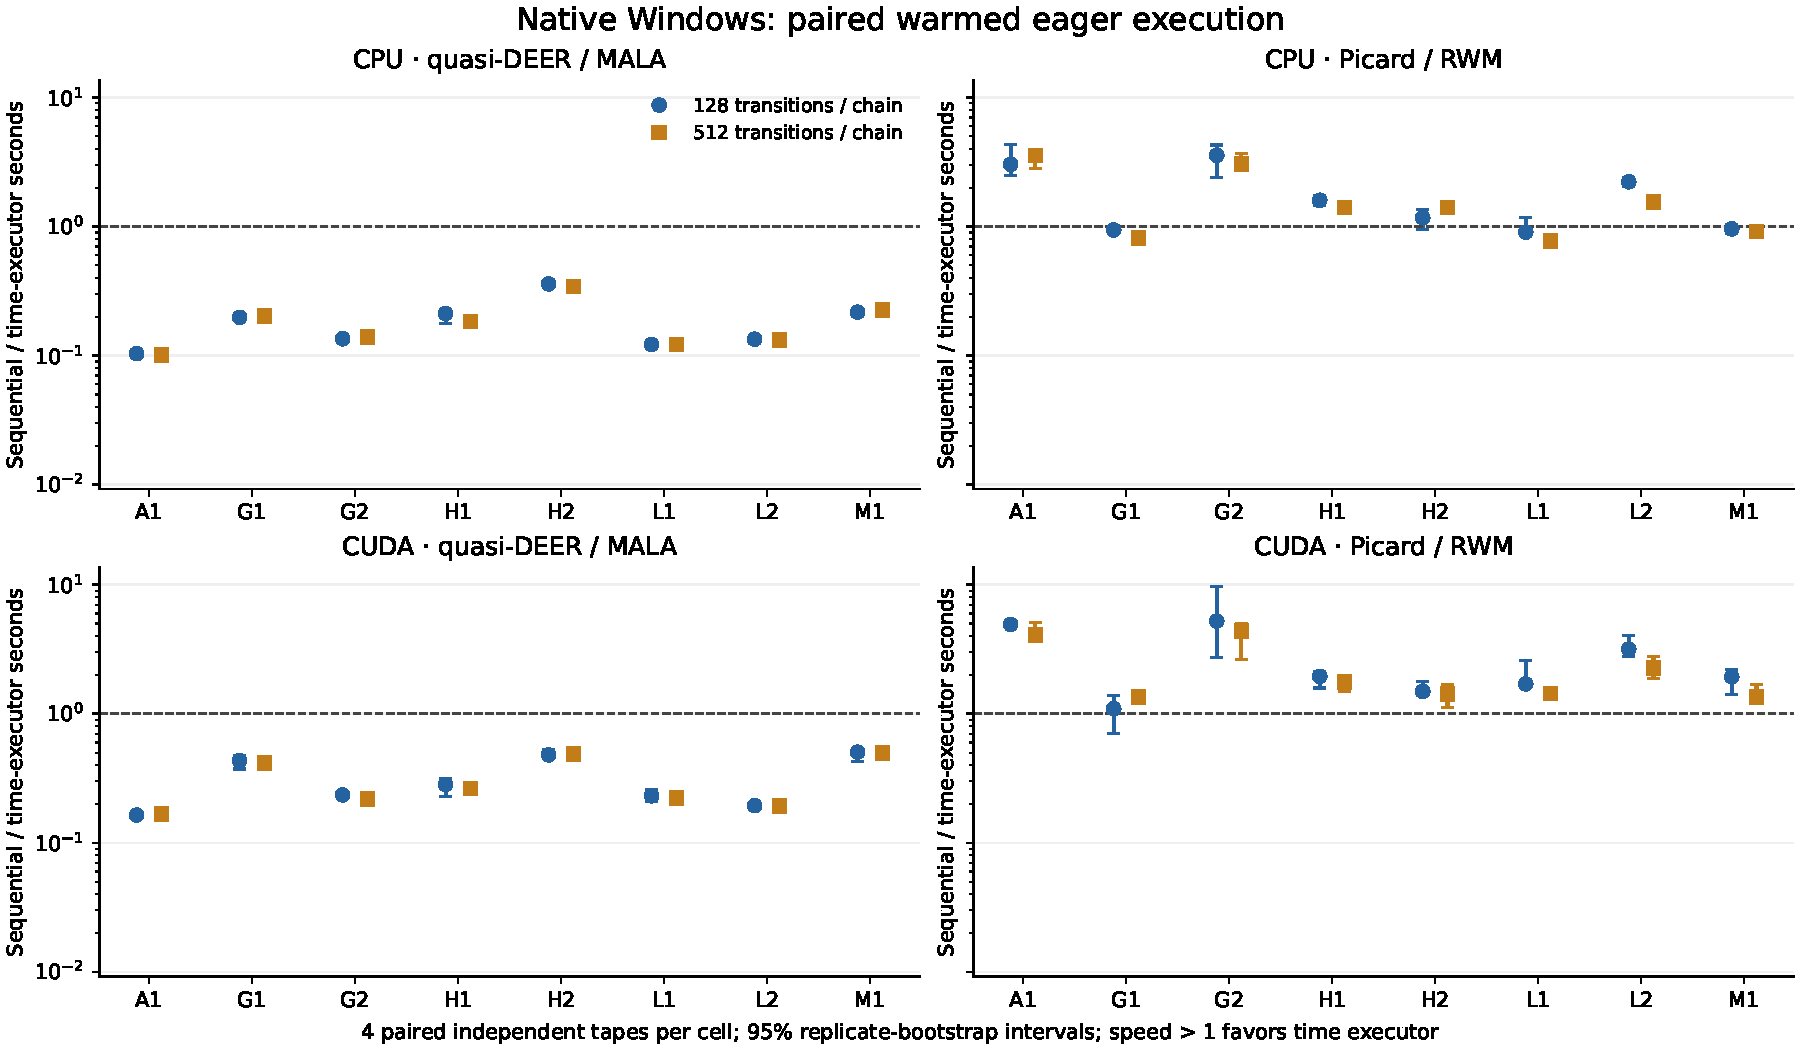
\includegraphics[width=\linewidth]{../../benchmark/analysis/outputs/windows-native-v1/speed-ratios.pdf}
\caption{原生Windows配对执行结果；每组4份独立数组，误差线为重复层面2000次bootstrap的逐点95\%区间，
不提供同时置信保证。CUDA Picard的@CUDA_PICARD_FASTER@组中位数大于1，其中@CUDA_PICARD_CI@组区间下限大于1。
A1/RWM的全部@NO_MOVE@次拟合均拒绝所有提议，其速度仅反映自环执行，不能解释为后验探索加速。
quasi-DEER的所有组中位速度比均小于1；全部负结果保留。}
\end{figure}

数值完成与推断可靠性有明显区别：@RHAT_FITS@/@TASKS@次拟合至少有一个有限rank/folded Rhat大于1.01，
@CONSTANT_FITS@次拟合包含常量变量或函数，其诊断保留为不可判定。
最大有限Rhat为@RHAT_MAX@，最小有限bulk/tail ESS为@BULK_MIN@/@TAIL_MIN@。
该Rhat计数仅为描述，没有新增事后验收标准。解析目标的逐函数重复MSE及区间另行保存；
L1/L2的有限参考未解决，不宣称精度达标。全拒绝或混合不足轨迹没有被删除或重新调参替换。

另以12个新生成数据集进行小型SBC，五个共享数据工作流共60次拟合全部完成。
同数据解析90\%区间与五个工作流的覆盖均为9/12，解析覆盖的95\%区间为[0.428,0.945]；
端点、矩和诊断分别保存。共享数据不能计作60个独立校准重复。
Pyro CPU NUTS与MH不使用固定同轨迹比较，也未纳入本轮正式速度实验。

正式任务记录成本共@ATTEMPT_SECONDS@秒（含普通执行和技术重放），现代R诊断另计@DIAGNOSTIC_SECONDS@秒；
普通API包括建模和基本矩；核验API使用已构建模型，包含独立参考但不含建模和基本矩。
建模、写盘与现代诊断分别记录，这些计时不能混称完整工作流。
最大CUDA分配/保留峰值为@CUDA_ALLOCATED@/@CUDA_RESERVED@字节，包含已有驻留分配；
CPU仅有数组空间估算，未测逐拟合RSS峰值。主机标量读取累计@SCALAR_READS@次，
标量等待计时@SCALAR_SECONDS@秒含设备等待，并不隔离全部控制开销。
试探分析曾把共享数组的配置变化合并为误差区间；该区间已撤回，原输出及哈希保留，正式分析不受影响。
本轮结果仅支持指定Windows实现和有限预算下的计算证据，不将Mac JAX与Windows torch的完整工作流差异全部归因于GPU。


\paragraph{回传后的独立复核。}
Mac端校验归档内5866个文件，使用冻结NumPy参考重放128条四链配置并核对全部512项实际数组；
接受事件仍为零失配，同设备速度比和逐函数误差可由原始记录重建。
复算512项正式及60项SBC的现代诊断时发现十进制读取敏感性：
NumPy读取的参数列与保存数组逐值相同，但Mac R直接读取CSV会改变部分接近重复值的末位精度。
以小端float64二进制传入R后，在绝对及相对$10^{-11}$比较容差下，
正式诊断的数值分歧由4158个指标值降至2个，SBC由31个降至0个。
剩余2个Rhat差异约为$3.46\times10^{-4}$；后续最小复现定位的数值机制见第\ref{sec:completion-companion}节。
@RHAT_FITS@项Rhat偏高和@CONSTANT_FITS@项常量输出的计数保持不变。
这是新增的伴随敏感性分析，保留Windows原诊断，不将数值接近的路径等同于秩诊断逐值可复现。
该复核没有重新测量GPU性能，也没有扩大已验证后端范围。
